\chapter{Diseño e Implementación} % Main chapter title

\label{Chapter3} % Change X to a consecutive number; for referencing this chapter elsewhere, use \ref{ChapterX}
\definecolor{mygreen}{rgb}{0,0.6,0}
\definecolor{mygray}{rgb}{0.5,0.5,0.5}
\definecolor{mymauve}{rgb}{0.58,0,0.82}

%----------------------------------------------------------------------------------------

La idea de esta sección es resaltar los problemas encontrados, los criterios utilizados y la justificación de las decisiones que se hayan tomado.

\section{Hardware}

\begin{figure}[h]
	\centering
	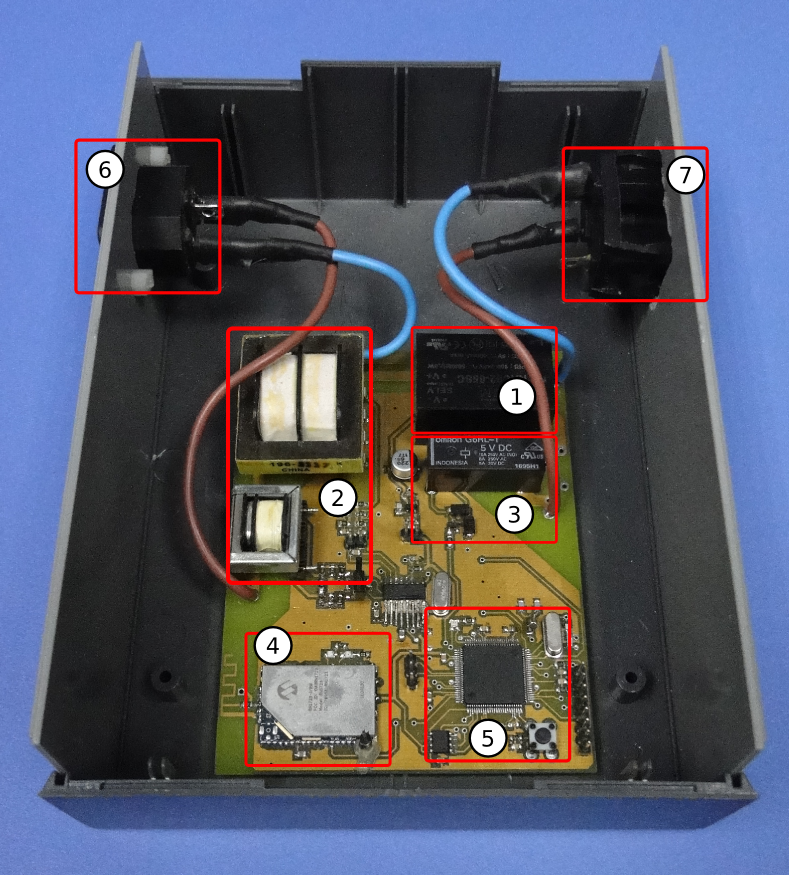
\includegraphics[width=10cm]{./Figures/3_1_prototipo_1.png}
	\caption{Prototipo funcional del Smart Plug.}
	\label{fig:prototipo}
\end{figure}

\subsection{Esquemático general}

\begin{figure}[h]
	\centering
	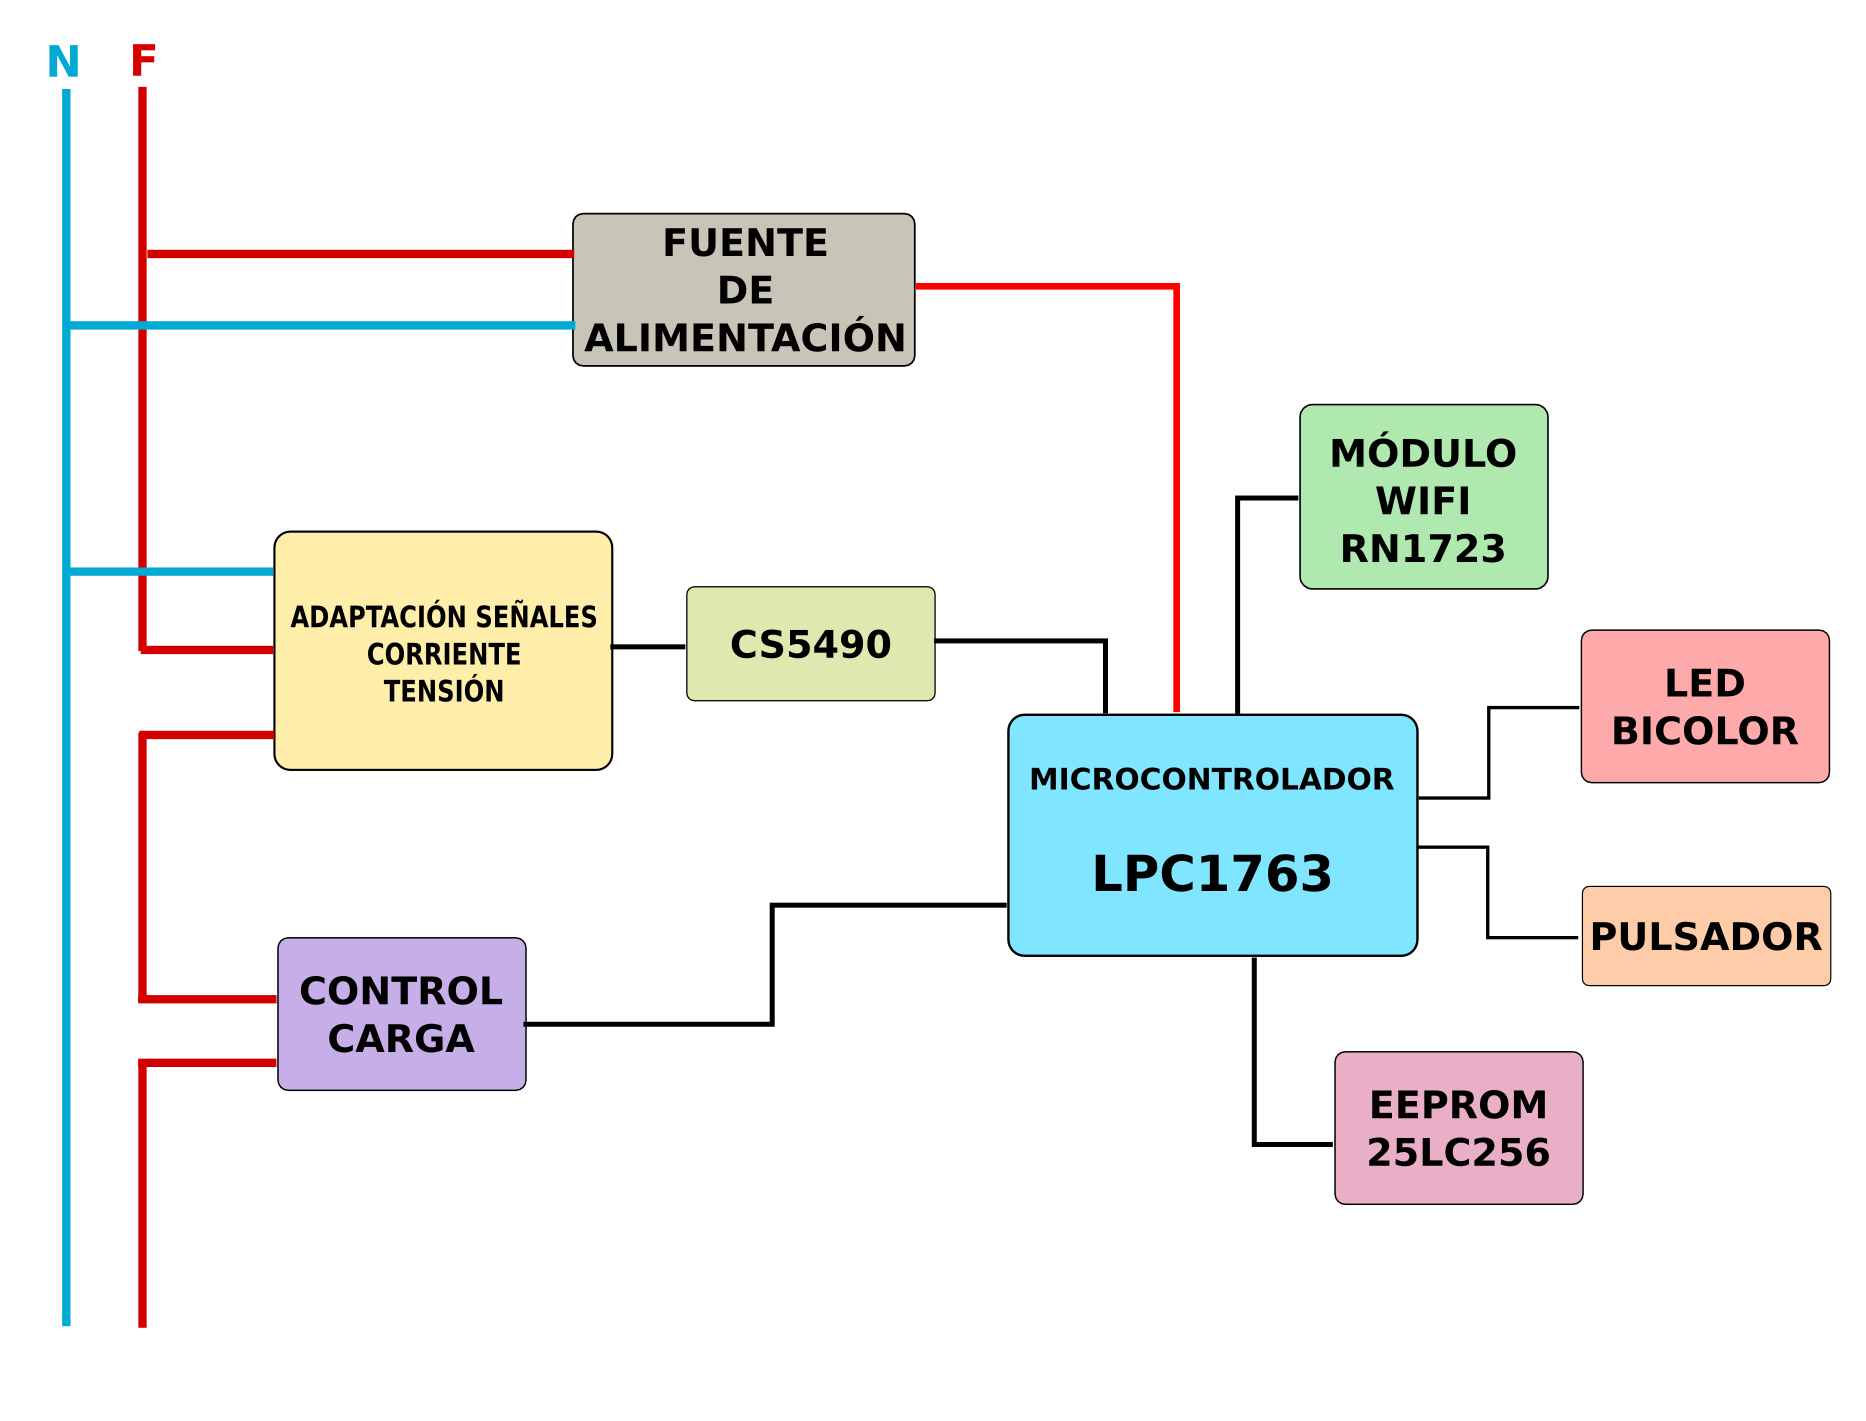
\includegraphics[width=12cm]{./Figures/3_1_1_diagrama_bloques_hardware.png}
	\caption{Diagrama en bloques del hardware del prototipo funcional.}
	\label{fig:hardware_diagrama_bloques}
\end{figure}

\subsection{Detalles de los módulos de hardware}

\begin{figure}[h]
	\centering
	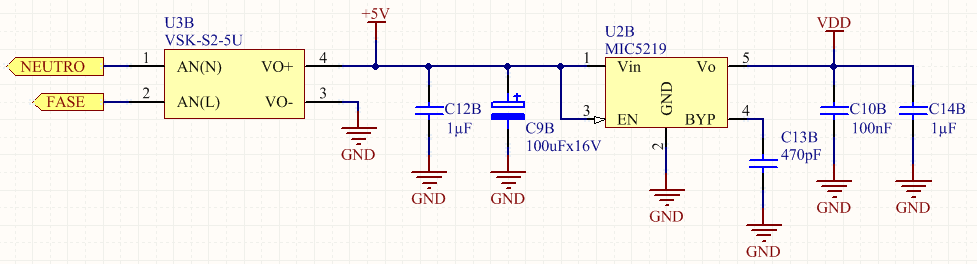
\includegraphics[width=14cm]{./Figures/3_1_2_pcb_fuente.png}
	\caption{Esquemático de la fuente de alimentación.}
	\label{fig:pcb_fuente}
\end{figure}

\begin{figure}[h]
	\centering
	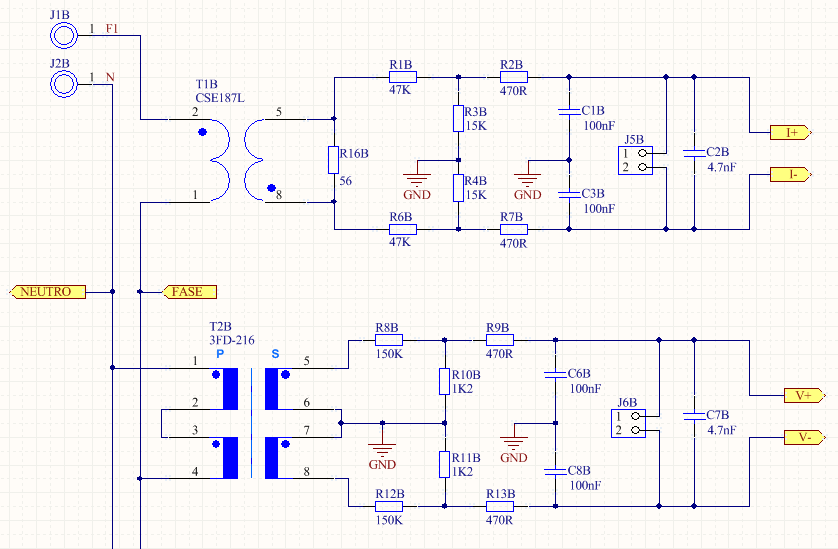
\includegraphics[width=14cm]{./Figures/3_1_2_pcb_adaptacion.png}
	\caption{Esquemático de la etapa de adaptación de las señales de tensión y corriente de la línea eléctrica.}
	\label{fig:pcb_adaptacion}
\end{figure}

\begin{figure}[h]
	\centering
	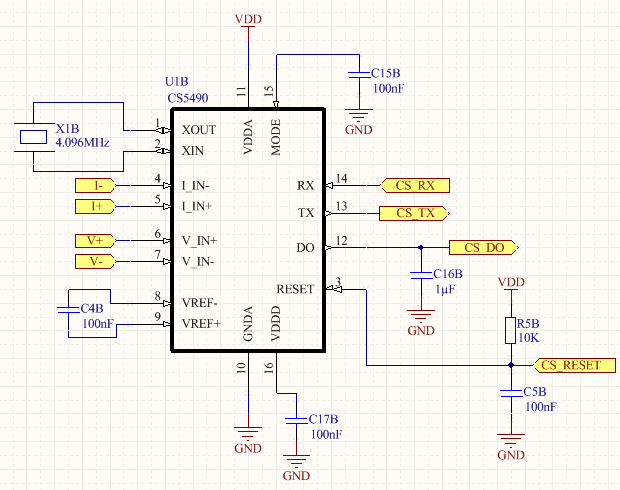
\includegraphics[width=14cm]{./Figures/3_1_2_pcb_medicion_energia.png}
	\caption{Esquemático del front-end analógico encargado de medir los parámetros eléctricos.}
	\label{fig:pcb_medicion_energia}
\end{figure}

\begin{figure}[h]
	\centering
	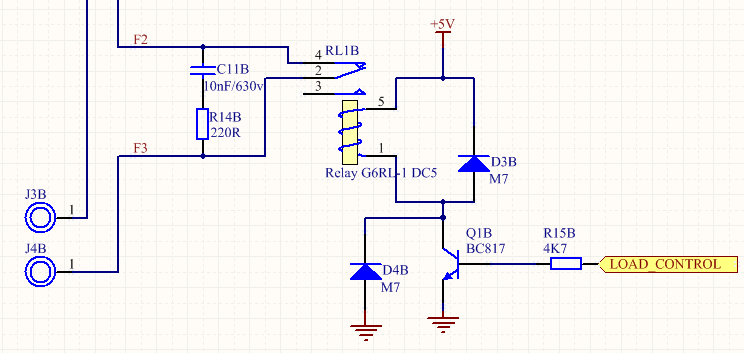
\includegraphics[width=10cm]{./Figures/3_1_2_pcb_control_carga.png}
	\caption{Esquemático del control de la carga eléctrica mediante un relay mecánico.}
	\label{fig:pcb_control_carga}
\end{figure}

\begin{figure}[h]
	\centering
	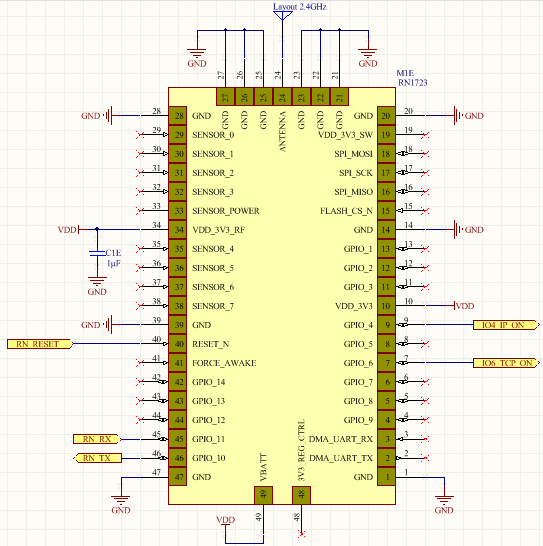
\includegraphics[width=12cm]{./Figures/3_1_2_pcb_wifi.png}
	\caption{Esquemático del módulo WiFi.}
	\label{fig:pcb_wifi}
\end{figure}


\section{Firmware}

\subsection{Arquitectura del firmware}

\begin{figure}[h]
	\centering
	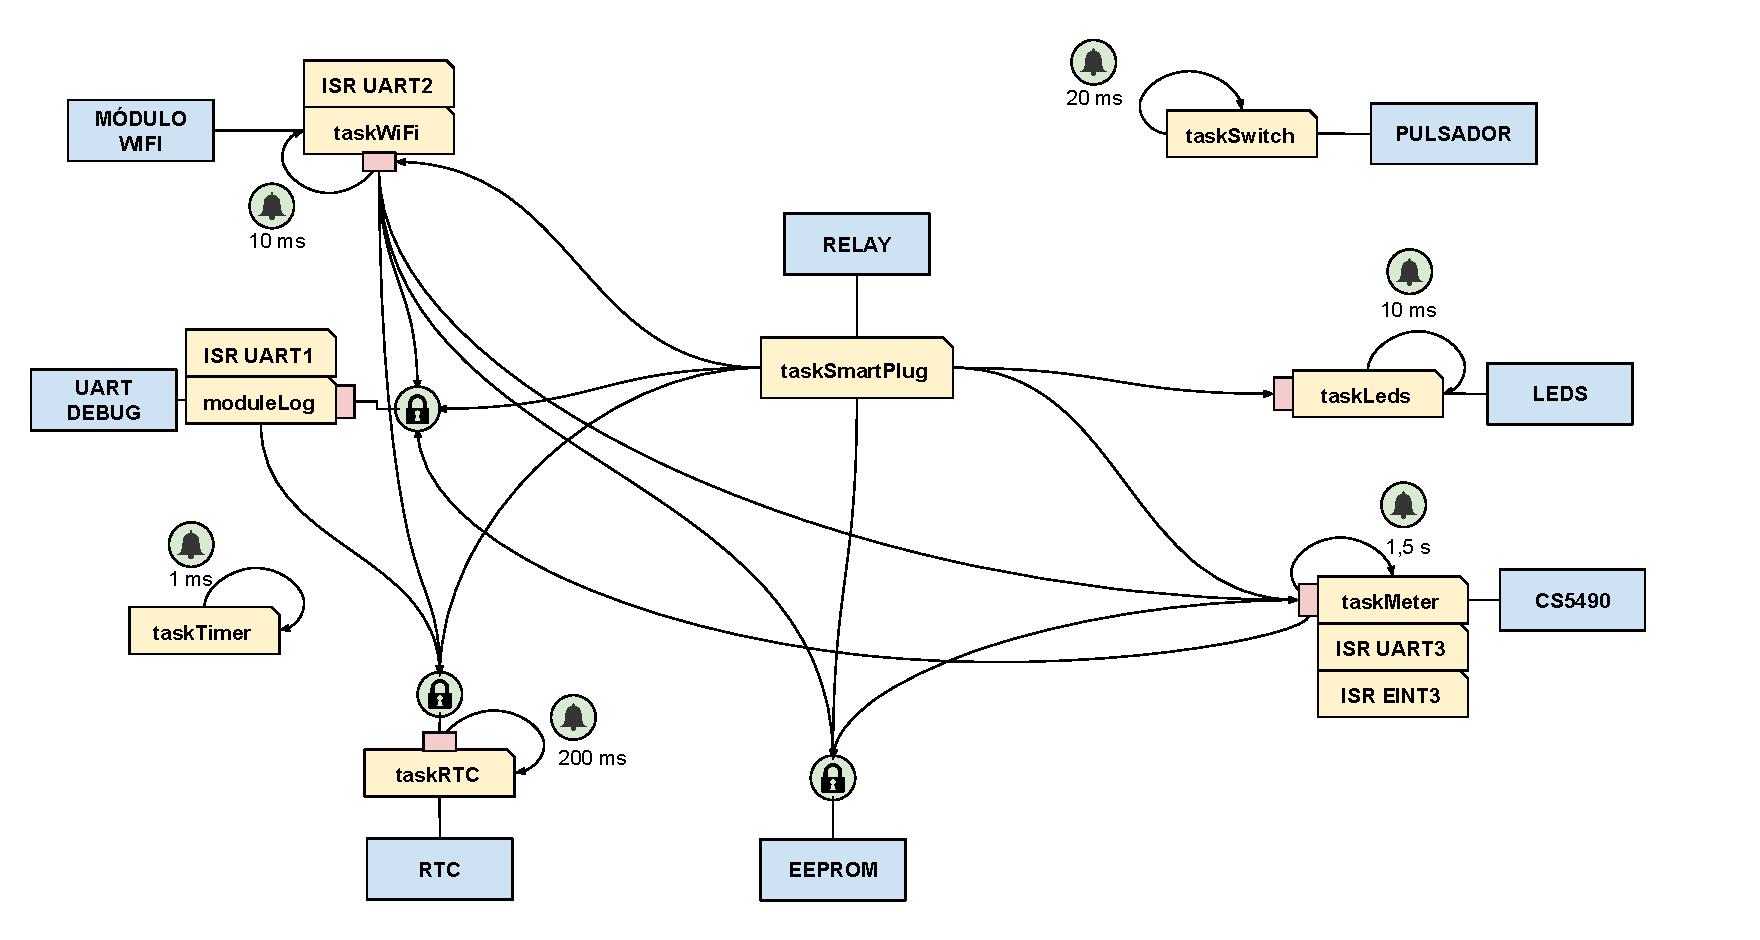
\includegraphics[width=16cm]{./Figures/3_2_1_firmware_esquema_tareas.pdf}
	\caption{Esquema de las tareas y recursos utilizados en el firmware.}
	\label{fig:firmware_esquema_tareas}
\end{figure}


\subsection{Capas de abstracción}

\begin{figure}[h]
	\centering
	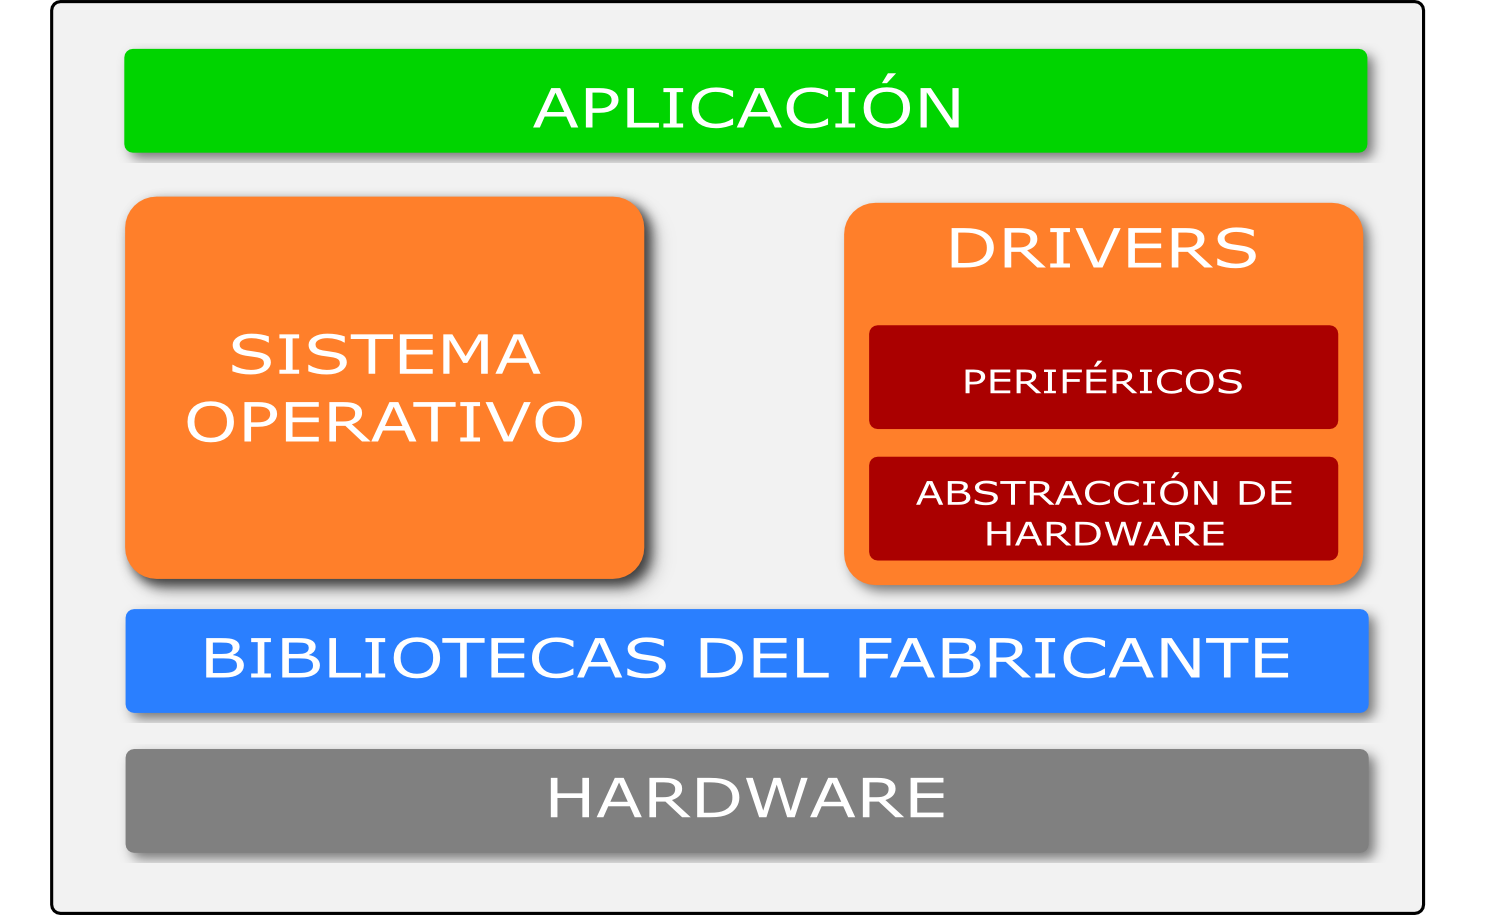
\includegraphics[width=10cm]{./Figures/3_2_2_firmware_diagrama_capas.png}
	\caption{Capas del firmware.}
	\label{fig:firmware_diagrama_capas}
\end{figure}


\subsection{Metodología orientada a objetos}

\begin{figure}[h]
	\centering
	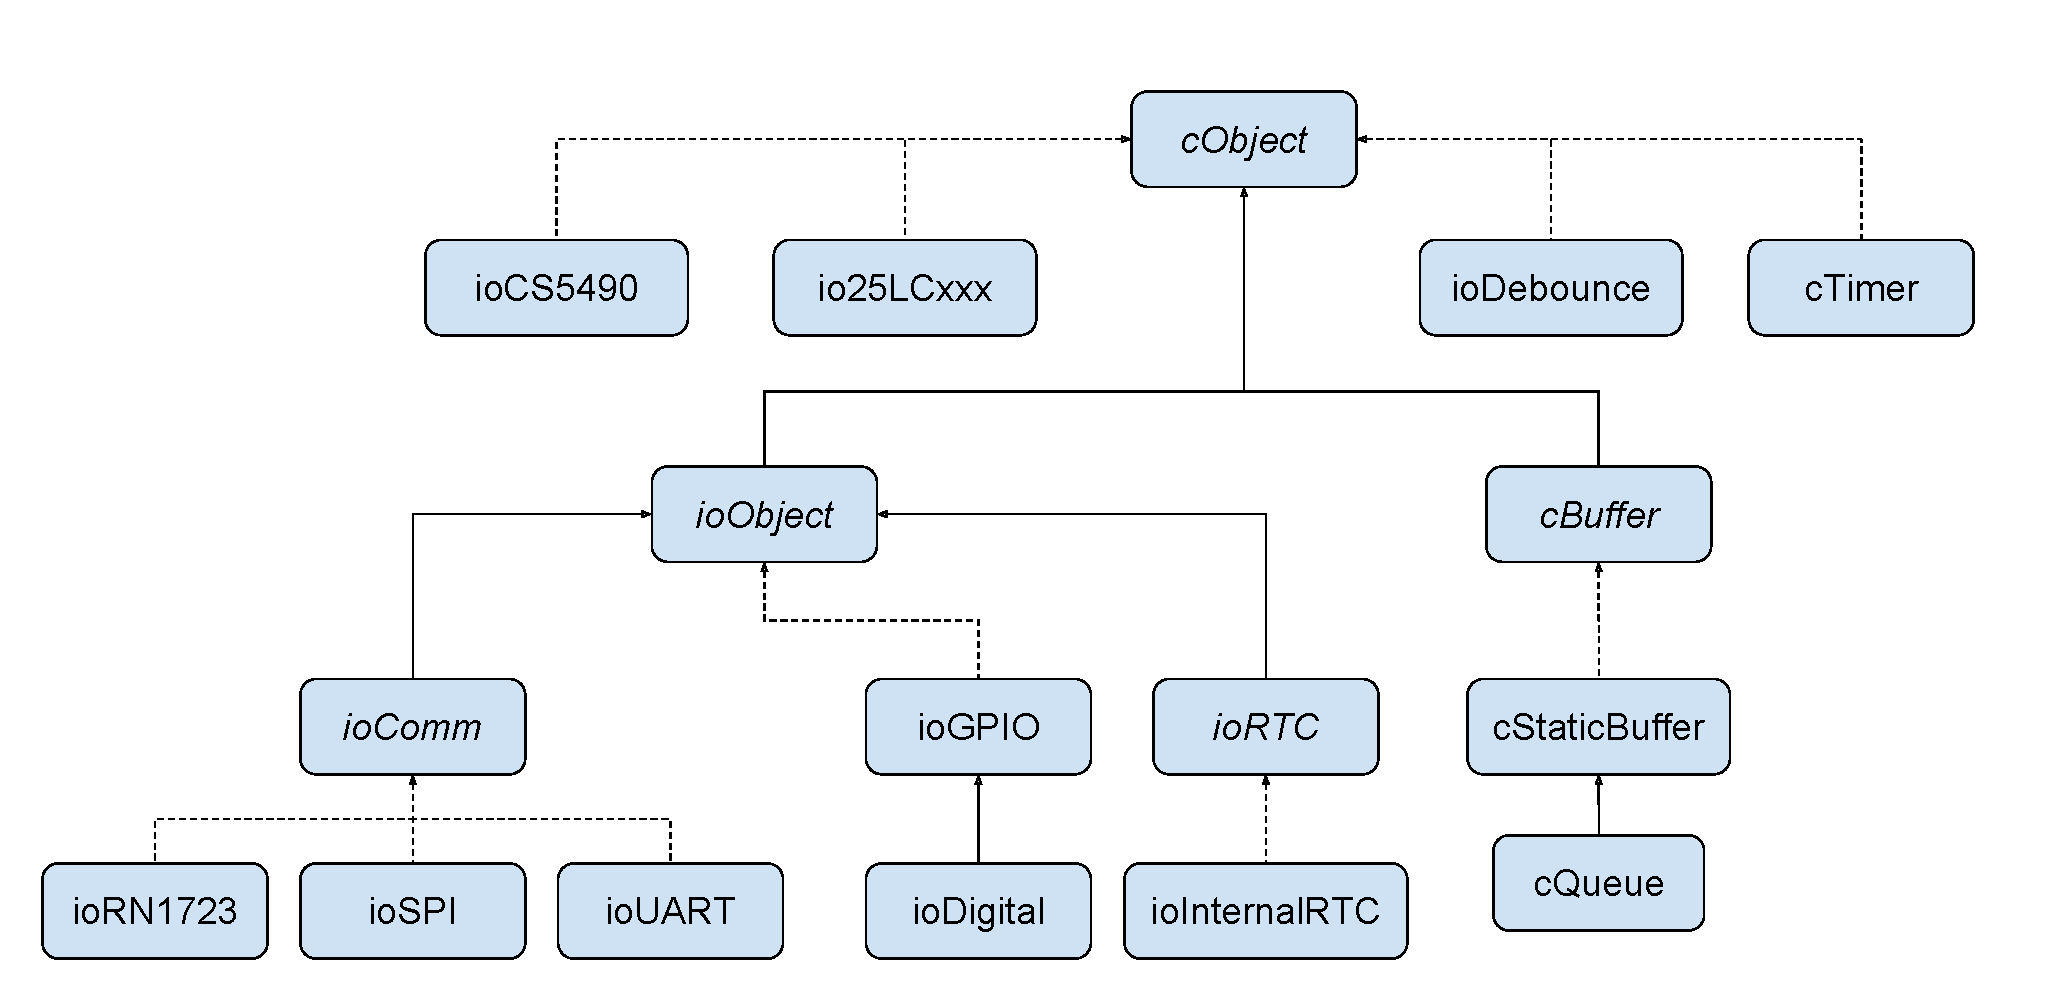
\includegraphics[width=14cm]{./Figures/3_2_3_diagrama-clases-simplificado.pdf}
	\caption{Diagrama de clases de los controladores desarrollados para el firmware.}
	\label{fig:firmware_diagrama_clases}
\end{figure}


\subsection{Protocolo de comunicación}

\begin{figure}[h]
	\centering
	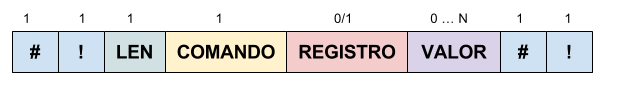
\includegraphics[width=12cm]{./Figures/3_2_4_formato_trama.pdf}
	\caption{Formwato de la trama.}
	\label{fig:formato_trama}
\end{figure}


\subsection{Uso de los comandos}

\begin{figure}[h]
	\centering
	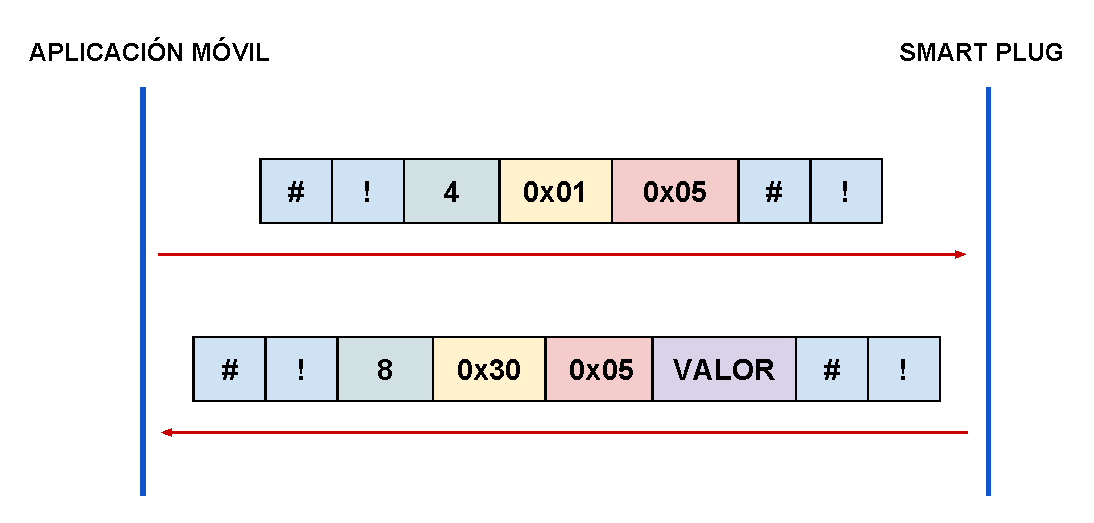
\includegraphics[width=12cm]{./Figures/3_2_5_comunicacion_GET.pdf}
	\caption{Diagrama de comunicación del comando \textit{GET}.}
	\label{fig:comunicacion_get}
\end{figure}


\begin{figure}[h]
	\centering
	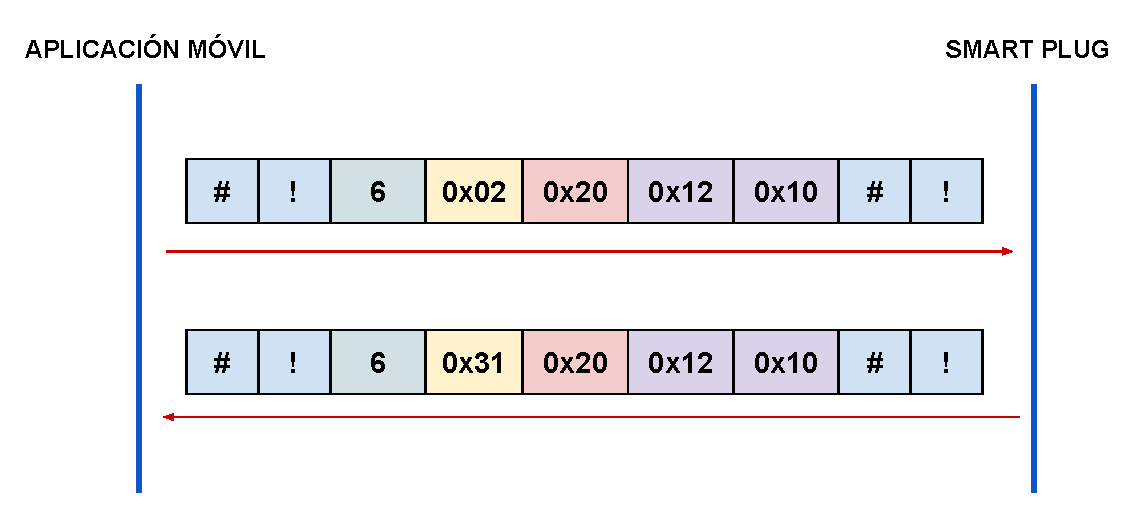
\includegraphics[width=12cm]{./Figures/3_2_5_comunicacion_SET.pdf}
	\caption{Diagrama de comunicación del comando \textit{SET}.}
	\label{fig:comunicacion_set}
\end{figure}


\begin{figure}[h]
	\centering
	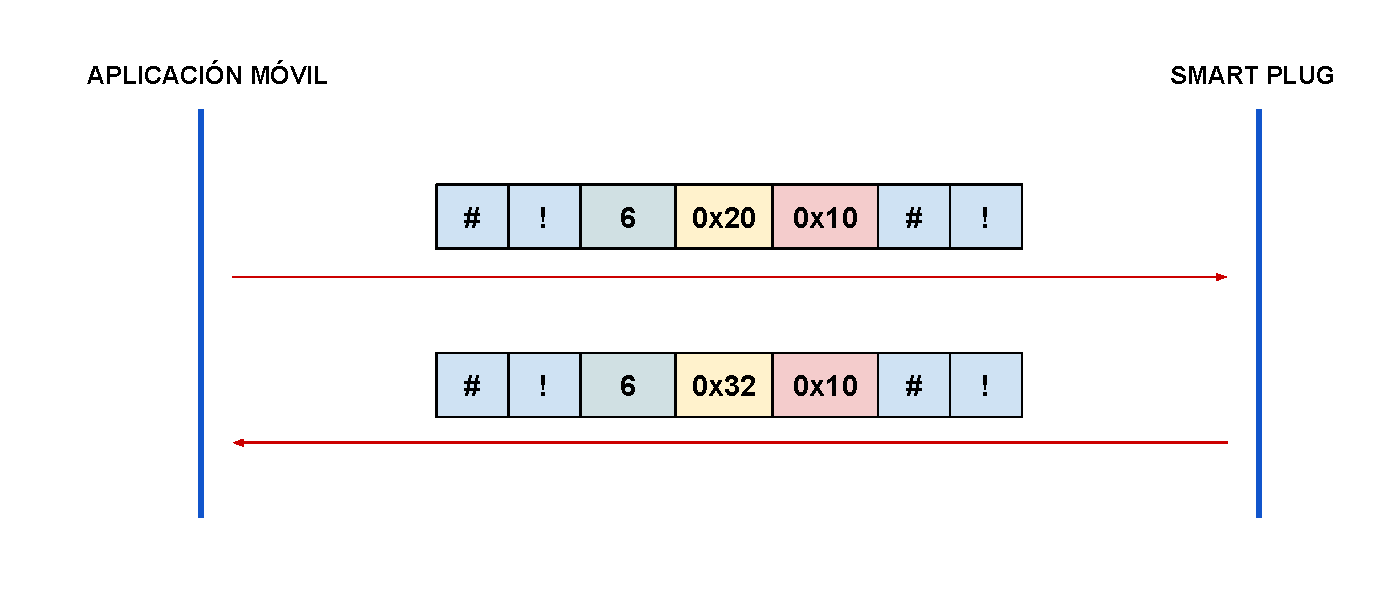
\includegraphics[width=12cm]{./Figures/3_2_5_comunicacion_RESET.pdf}
	\caption{Diagrama de comunicación del comando \textit{RESET}.}
	\label{fig:comunicacion_reset}
\end{figure}


\begin{figure}[h]
	\centering
	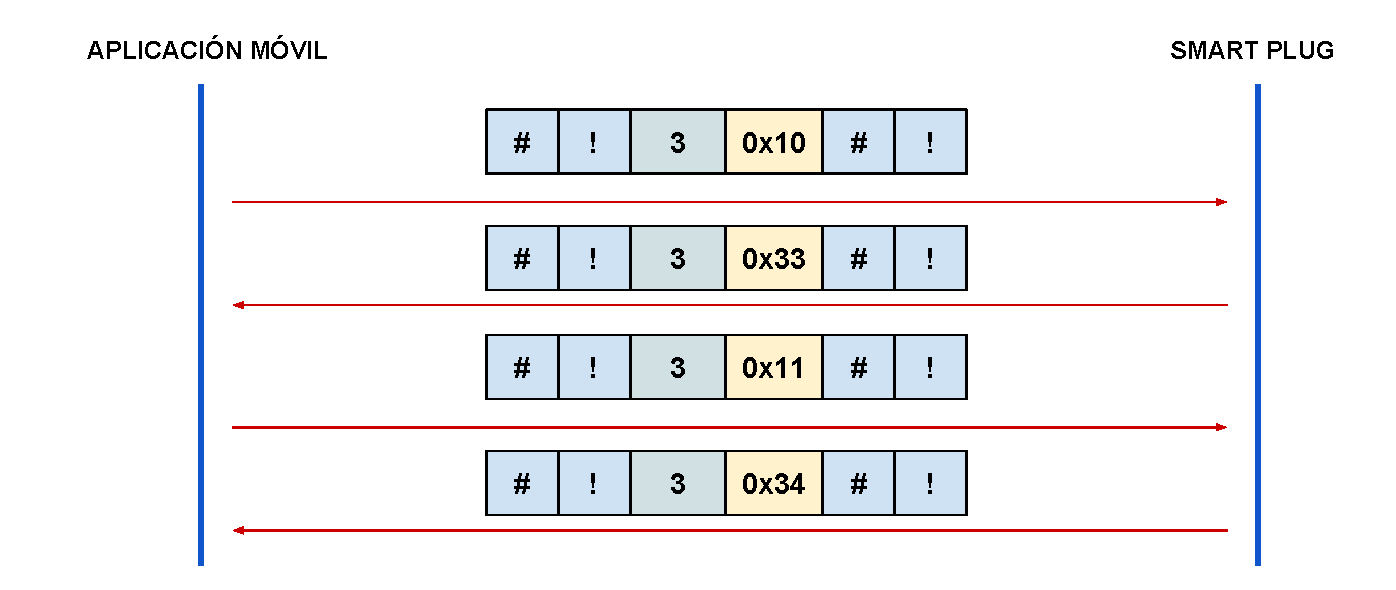
\includegraphics[width=12cm]{./Figures/3_2_5_comunicacion_NODE.pdf}
	\caption{Diagrama de comunicación de los comandos \textit{NODE ON} y \textit{NODE OFF}.}
	\label{fig:comunicacion_node}
\end{figure}


\section{Aplicación Android}

\subsection{Maqueta de la aplicación}

\begin{figure}[h]
	\centering
	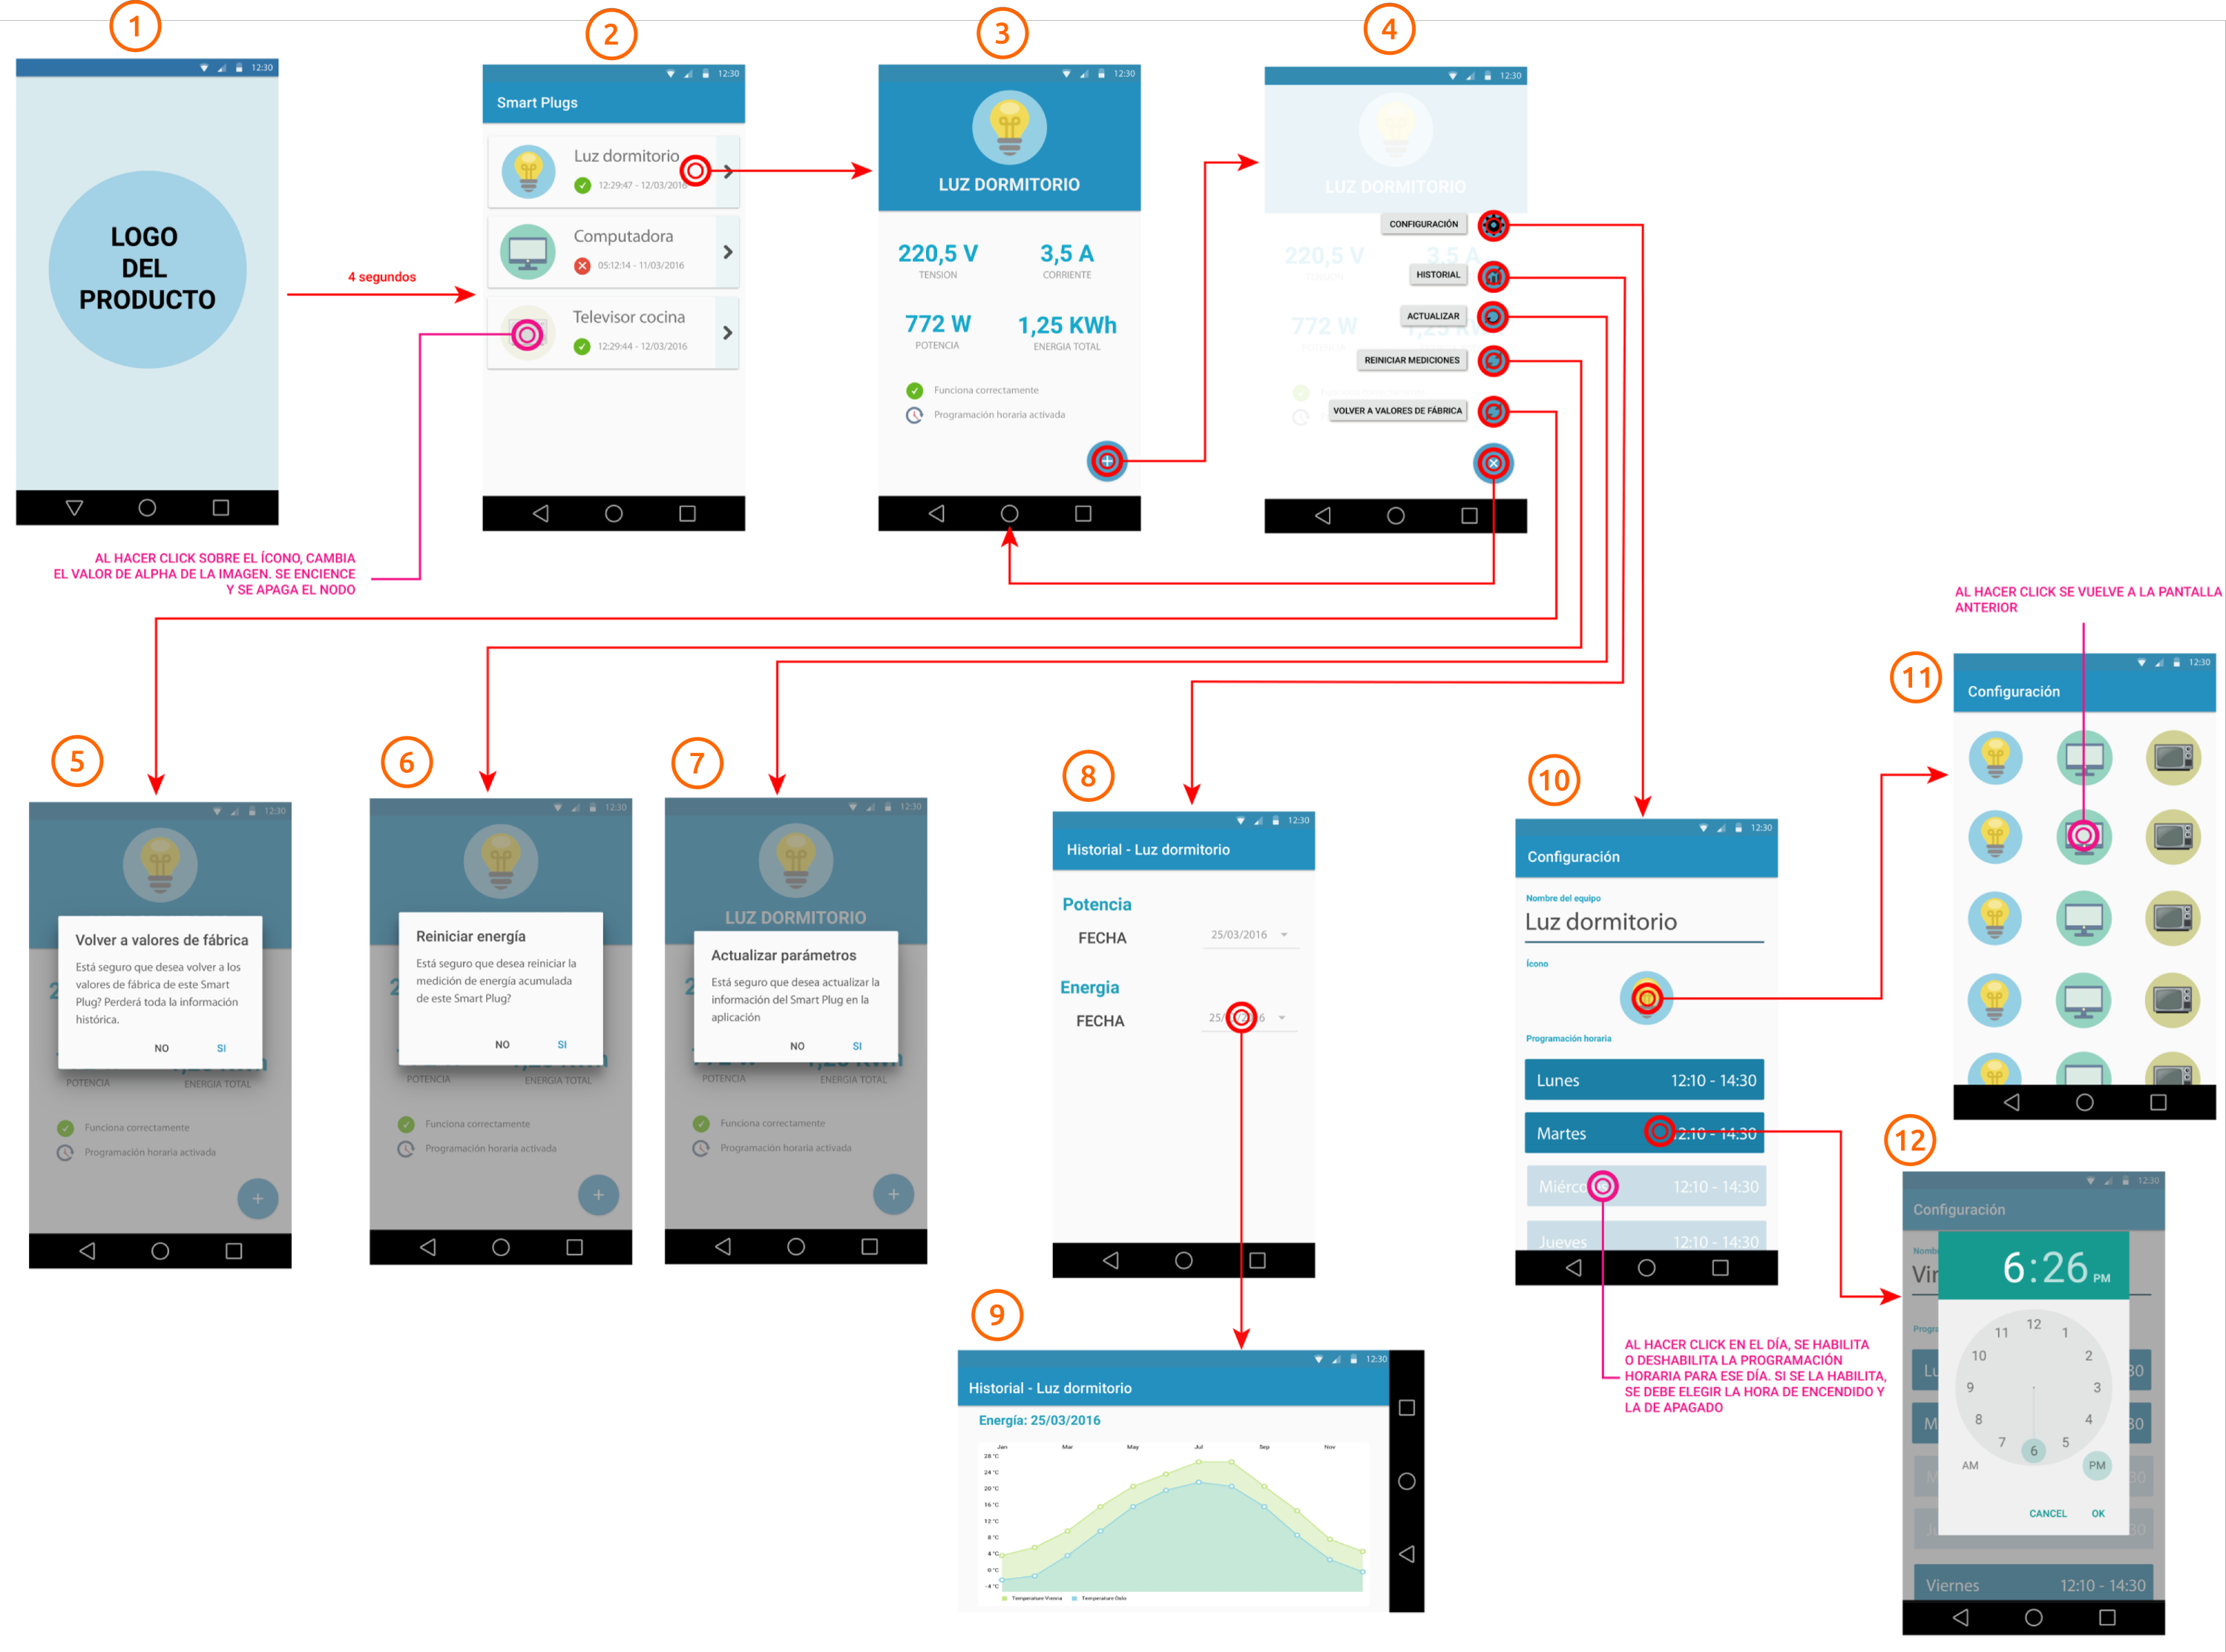
\includegraphics[width=18cm, angle=90]{./Figures/3_3_1_app_wireframe.png}
	\caption{Maqueta de la aplicación móvil.}
	\label{fig:comunicacion_app_wireframe}
\end{figure}


\subsection{Arquitectura de la aplicación}

\begin{figure}[h]
	\centering
	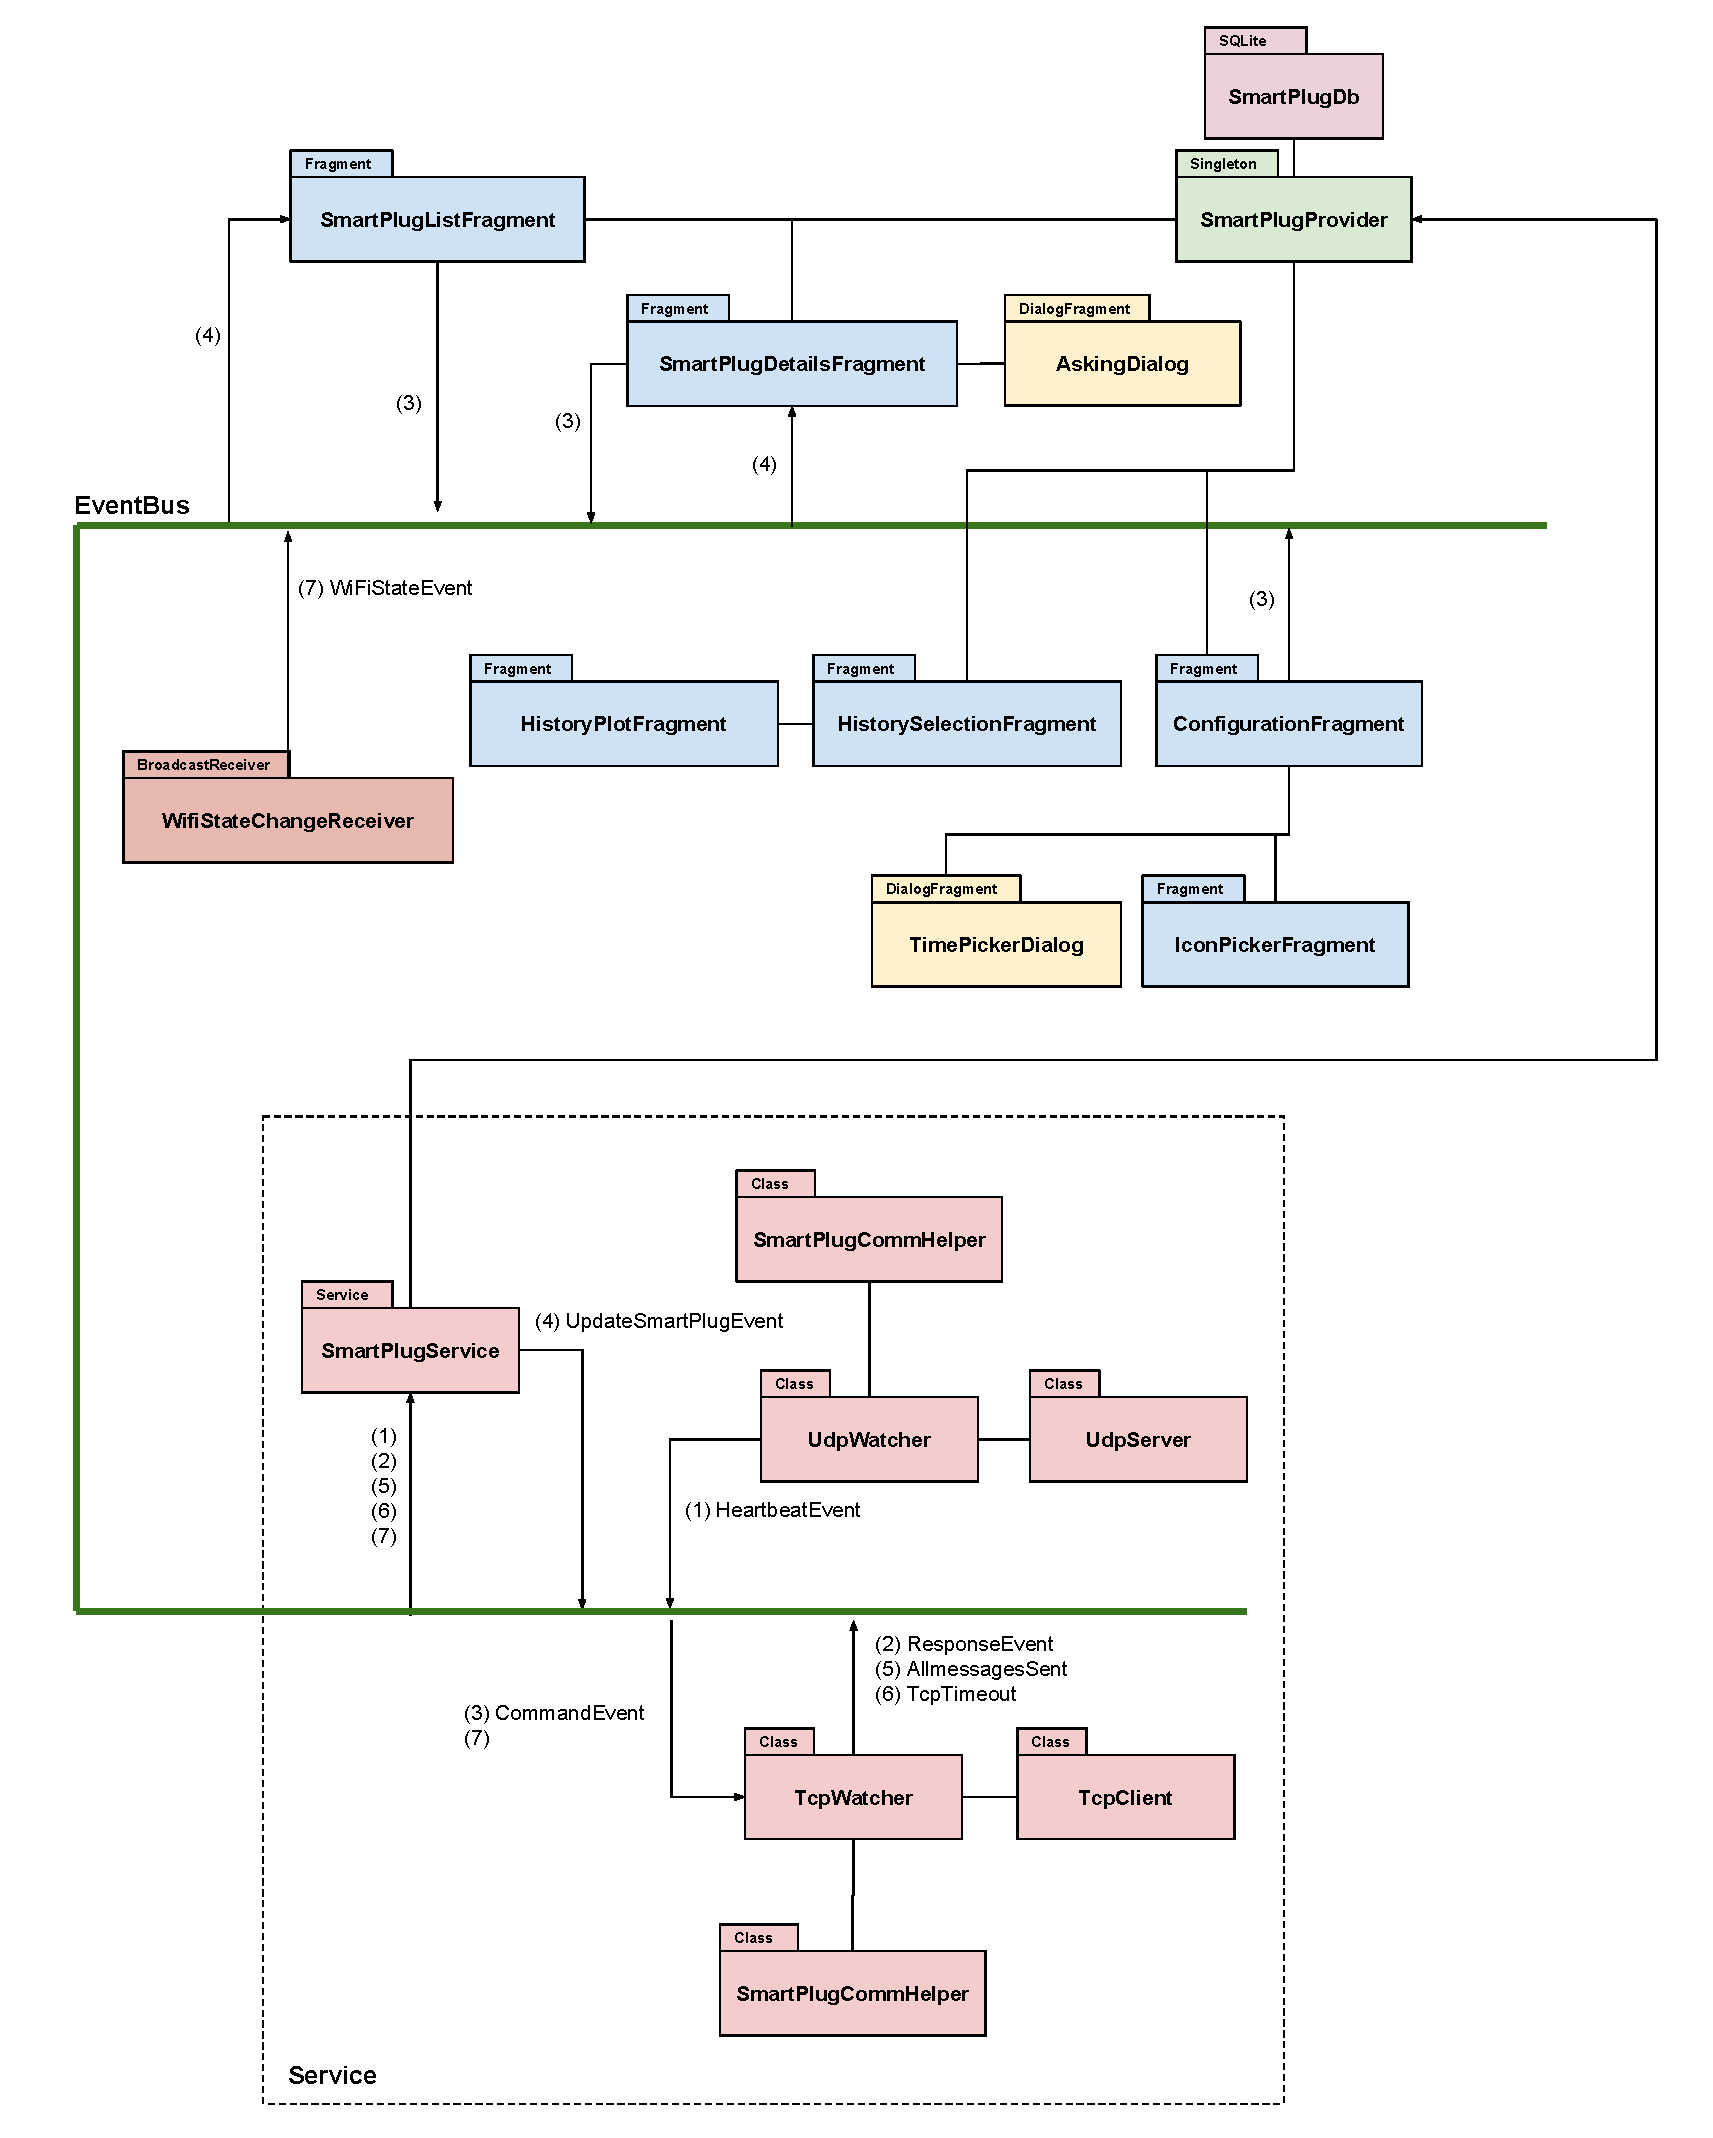
\includegraphics[width=14cm]{./Figures/3_3_2_app-arquitectura.pdf}
	\caption{Relación entre las clases desarrolladas para la aplicación móvil.}
	\label{fig:app_arquitectura}
\end{figure}



